\documentclass[a4paper,10pt]{report}
\usepackage{geometry}\geometry{a4paper,top=3.5cm,bottom=3.5cm,%
left=2.5cm,right=2.5cm,heightrounded,bindingoffset=0mm}
\usepackage[T1]{fontenc}
\usepackage[utf8]{inputenc}
\usepackage[italian]{babel}
\usepackage{graphicx}
\usepackage[export]{adjustbox}%Per il Frame attrono le immagini e il valign
\usepackage{subfig}
\usepackage{amsmath,amsfonts,amssymb,braket,mathrsfs}
\usepackage{float}
\usepackage{tabularx,booktabs}
\usepackage{hyperref}
\usepackage{epsfig}
\usepackage{pdfpages} %Per gli allegati
%\usepackage{minipage}
\usepackage[output-decimal-marker={,}]{siunitx}
\DeclareSIUnit \days {gg}
%ILe tre righe sotto ervono per mettere il grassetto dentro la tabelle siunitex usando \B, il rosso usando \RED, e il verde usando \GREEN
\sisetup{detect-weight,mode=text}
\usepackage{etoolbox}
\newrobustcmd\B{\DeclareFontSeriesDefault[rm]{bf}{b}\bfseries}
\newrobustcmd\RED{\DeclareFontSeriesDefault[rm]{bf}{b}\color{red}}
\newrobustcmd\GREEN{\DeclareFontSeriesDefault[rm]{bf}{b}\color{myGreen}}
%%
\usepackage{tikz}
\usepackage{pgfplots,pgfplotstable}
%\pgfplotsset{compat=1.15} %indica la versione da utilizzare per pgfplot
\usetikzlibrary{patterns} % per il tratteggio
\usepgfplotslibrary{groupplots}
\pgfplotsset{compat=newest}
%\usepackage{stanli}
\usepackage{xspace}% per lo spazio intelligente
\newcommand{\e}{\`E\xspace}  %E'
\usepackage{titlesec} % per formato custom dei titoli dei capitoli
%\usepackage{sideways}%%%
% redefinizione del formato del titolo del capitolo
      % da formato
      %   Capitolo X
      %   Titolo capitolo
      %   a formato
      %      Titolo capitolo 
	\titleformat{\chapter}
        {\normalfont\Huge\bfseries}{}{0em}{}
	\titlespacing*{\chapter}{0pt}{0in}{0.02in}
	\titlespacing*{\section}{0pt}{0.2in}{0.02in}
	\titlespacing*{\subsection}{0pt}{0.10in}{0.02in}
%serve per la didascalia di tabelle e figure:
\usepackage{caption}
\captionsetup{tableposition=top,figureposition=bottom,font=small}\captionsetup{format=hang,labelfont={bf,color=pantone186}} %didascalie a più righe allineate e il nome in grassetto
%non viene allineato a sinistra se la didascalia è corta una sola riga. PERCHé??
\usepackage{xcolor}
%serve per mettere il codice con lo sfondo grigio chiaro
\definecolor{pantone186}{RGB}{206, 17, 38} %il colore del logo UNITN
\definecolor{myGray}{gray}{0.5} %più basso più scuro è
\definecolor{myGreen}{rgb}{0.0, 0.5, 0.0}
\usepackage{listings} 
\lstset{basicstyle=\scriptsize\ttfamily,
backgroundcolor=\color{lightgray},%
boxpos=c,%
stringstyle=\itshape,		
lineskip=3pt,%
numbers=left,
numberstyle=\tiny,}
\usepackage{lscape}
\usepackage{multirow}
\usepackage{import}
%\usepackage{pythontex}
\begin{document}
%!TEX root = ../TesiTriennaleMeoliNicola.tex
\pagestyle{plain}
\thispagestyle{empty}
\begin{center}
  \begin{figure}[H]
    \centerline{
\psfig{file=IMG/logo_unitn_black_centerNEW.eps,
                        width=0.8\textwidth,trim = 0 0.9cm 0 0.5cm}}
  \end{figure}
\textcolor{pantone186}{\noindent\rule{\textwidth}{.5pt}}

  \Large\textsc{Dipartimento di Ingegneria Civile, Ambientale e Meccanica\\}
  \Large{Corso di Laurea in Ingegneria Civile
  }

  \vspace{3.7 cm} 
  %\Large\textsc{Elaborato finale\\} 
  %\vspace{1 cm} 
  \Huge\textsc{Confronto energetico tra diverse soluzioni edilizie\\}
  
  \vspace{0.2 cm}
  \Large{\it{Analisi termo igrometrica di alcuni pacchetti strutturali composti da differenti materiali. }}


  \vspace{4 cm} 
  \begin{tabular*}{\textwidth}{ l @{\extracolsep{\fill}} r }
  \Large\textsc{Docenti} & \Large\textsc{Studente}\\
  \Large{Rossano Albatici}& \Large{Nicola Meoli 186100}\\
  
  	
  	
  \end{tabular*}

  \vspace{3.1cm} 
  \textcolor{pantone186}{\noindent\rule{\textwidth}{1pt}}
    
  \Large{Anno accademico 2020/21}
  
\end{center}


\tableofcontents
%\setcounter{page}{1}
%Tabelle e figure sulla stessa pagina:
%Le aggiunge all'indice. phantomsection serve per non far casini con hyperref
\clearpage
\begingroup
   %\let\cleardoublepage\relax  % book
    \let\clearpage\relax        % report
        \listoftables
        \phantomsection
        \addcontentsline{toc}{chapter}{Elenco delle tabelle}
        %
        \listoffigures
        \phantomsection
        \addcontentsline{toc}{chapter}{Elenco delle figure}
\endgroup
%
%%%%%%%%%%
%Comandi aggiunti:
%%%%%%%%%%
\newcommand{\red}[1]{\textcolor{pantone186}{#1}}
%%%%%%%%%%%%%%%%%%%%%%%%%%%%%%%%%%
\newcommand{\TabellaNodi}[3]{%
\begin{table}[p]
        %\small
        \centering
        \caption{#1}
        \label{#2}
        \begin{tabular}{
                        c
                        c
                        S[table-format=2.2]
                        S[table-format=1.3]
                        S[table-format=1.3]
                        c
                        S[table-format=3.2]
                        S[table-format=3.2]
                        S[table-format=1.2]
                        }
            \toprule
            \multicolumn{1}{c}{\multirow{3}{*}{Condotta}} & \multicolumn{1}{c}{\multirow{3}{*}{Tratto}} & \multicolumn{1}{c}{Lunghezza}       & \multicolumn{1}{c}{Pendenza} & \multicolumn{1}{c}{Dislivello}      & \multicolumn{1}{c}{\multirow{3}{*}{Nodo}} & \multicolumn{1}{c}{Quota}           & \multicolumn{1}{c}{Quota}           & \multicolumn{1}{c}{MAX } \\
                                              &                                             & \multicolumn{1}{c}{condotta}       & \multicolumn{1}{c}{$i_G^{prog}$}             & \multicolumn{1}{c}{$\Delta h$}      &                                           & \multicolumn{1}{c}{fondo}      & \multicolumn{1}{c}{terreno}    & \multicolumn{1}{c}{depth}\\
                                              &                                             & \multicolumn{1}{c}{[\si{\metre}]} & \multicolumn{1}{c}{[--]}                 & \multicolumn{1}{c}{[\si{\metre}]} &                                           & \multicolumn{1}{c}{[\si{\metre}]} & \multicolumn{1}{c}{[\si{\metre}]} & \multicolumn{1}{c}{[\si{\metre}]}\\
        \midrule 
        \multicolumn{8}{c}{\textbf{Corso del Lavoro e della Scienza}} \\ 
        \input{#3} \\
        \bottomrule
        \end{tabular}%
        \end{table}
}
%%%%%%%%%%%%%%%%%%%%%%%%%%%%%%%%%%
\newcommand{\TabellaDiametriCondotte}[3]{%
\begin{table}[p]
        %\small
        \centering
        \caption{#1}
        \label{#2}
        \begin{tabular}{
                        c
                        c
                        S[table-format=3.2]
                        S[table-format=3.2]
                        S[table-format=1.3]
                        S[table-format=1.2]
                        S[table-format=1.1]
                        S[table-format=-1.1]}
            \toprule
            \multicolumn{1}{c}{\multirow{2}{*}{Condotta}} & \multicolumn{1}{c}{\multirow{2}{*}{A valle di}}&\multicolumn{1}{c}{Deflusso}&\multicolumn{1}{c}{Deflusso totale}&\multicolumn{1}{c}{$i_G$}&\multicolumn{1}{c}{$D_{prog}$}&\multicolumn{1}{c}{$D_{comm}$}&\multicolumn{1}{c}{Offset}\\
            & &\multicolumn{1}{c}{[\si{\litre\per\second}]}&\multicolumn{1}{c}{[\si{\litre\per\second}]}&\multicolumn{1}{c}{[--]}&\multicolumn{1}{c}{[\si{\metre}]}&\multicolumn{1}{c}{[\si{\metre}]}&\multicolumn{1}{c}{[\si{\metre}]}\\
        \midrule 
        \multicolumn{8}{c}{\textbf{Via Roberto da Sanseverino}} \\ 
        \input{#3} \\
        \bottomrule
        \end{tabular}%
        \end{table}
}
%%%%%%%%%%%%%%%%%%%%%%%%%%%%%%%%%%%%%%%%%%%%%%%%%%%%%%%%%%%%%
\newcommand{\TabellaVerificheLinkFLow}[3]{%
\begin{landscape}
\begin{table}[p] 
    \centering
    \caption{#1}
    \label{#2}
    \begin{tabular}{
        c
        S[table-format=1.1]
        S[table-format=3.2]
        c
        S[table-format=1.2]
        S[table-format=2.0]
        S[table-format=1.4]
        S[table-format=1.4]
        S[table-format=1.4]
        S[table-format=1.3]
        S[table-format=1.2]c
        @{}}
        \toprule
        \multicolumn{2}{c|}{} & \multicolumn{3}{c|}{Velocità} & \multicolumn{6}{c}{Riempimento e Autopulizia} \\
        \midrule
        %
        \multicolumn{1}{c}{\multirow{3}{*}{Condotta}} & \multicolumn{1}{c}{\multirow{2}{*}{Diametro}} & \multicolumn{1}{c}{Flusso}                     & \multicolumn{1}{c}{Ora max}        & \multicolumn{1}{c}{Massima}                    & \multicolumn{1}{c}{Riempimento}       & \multicolumn{1}{c}{$\vartheta = $ }    & \multicolumn{1}{c}{Raggio}          & \multicolumn{1}{c}{Pend.}       & \multicolumn{1}{c}{Pend.}            & \multicolumn{1}{c}{Tensione } \\
        %
                                                      &                                               & \multicolumn{1}{c}{massimo}                    & \multicolumn{1}{c}{flusso}         & \multicolumn{1}{c}{velocità}                   & \multicolumn{1}{c}{massimo $G$}       & \multicolumn{1}{c}{compl. di $\alpha$} & \multicolumn{1}{c}{idraulico $R_H$} & \multicolumn{1}{c}{fondo $i_F$} & \multicolumn{1}{c}{geometrica $i_G$} & \multicolumn{1}{c}{tangenziale $\tau$} \\
        %
                                                      & \multicolumn{1}{c}{[\si{\metre}]}           & \multicolumn{1}{c}{[\si{\litre\per\second}]} & \multicolumn{1}{c}{[\si{\hour}]} & \multicolumn{1}{c}{[\si{\metre\per\second}]} & \multicolumn{1}{c}{[\si{\percent}]} & \multicolumn{1}{c}{[\si{rad}]}       & \multicolumn{1}{c}{[\si{\metre}]} & \multicolumn{1}{c}{[--]}        & \multicolumn{1}{c}{[--]}             & \multicolumn{1}{c}{[\si{\pascal}]} \\
                                              \midrule
        \input{#3} \\
        \bottomrule
\end{tabular}%
\end{table}
\end{landscape}
}
%%%%%%%%%%%%%%%%%%%%%%%
\chapter{nome capitlo 1}
\begin{figure}[htbp]
    \centering
    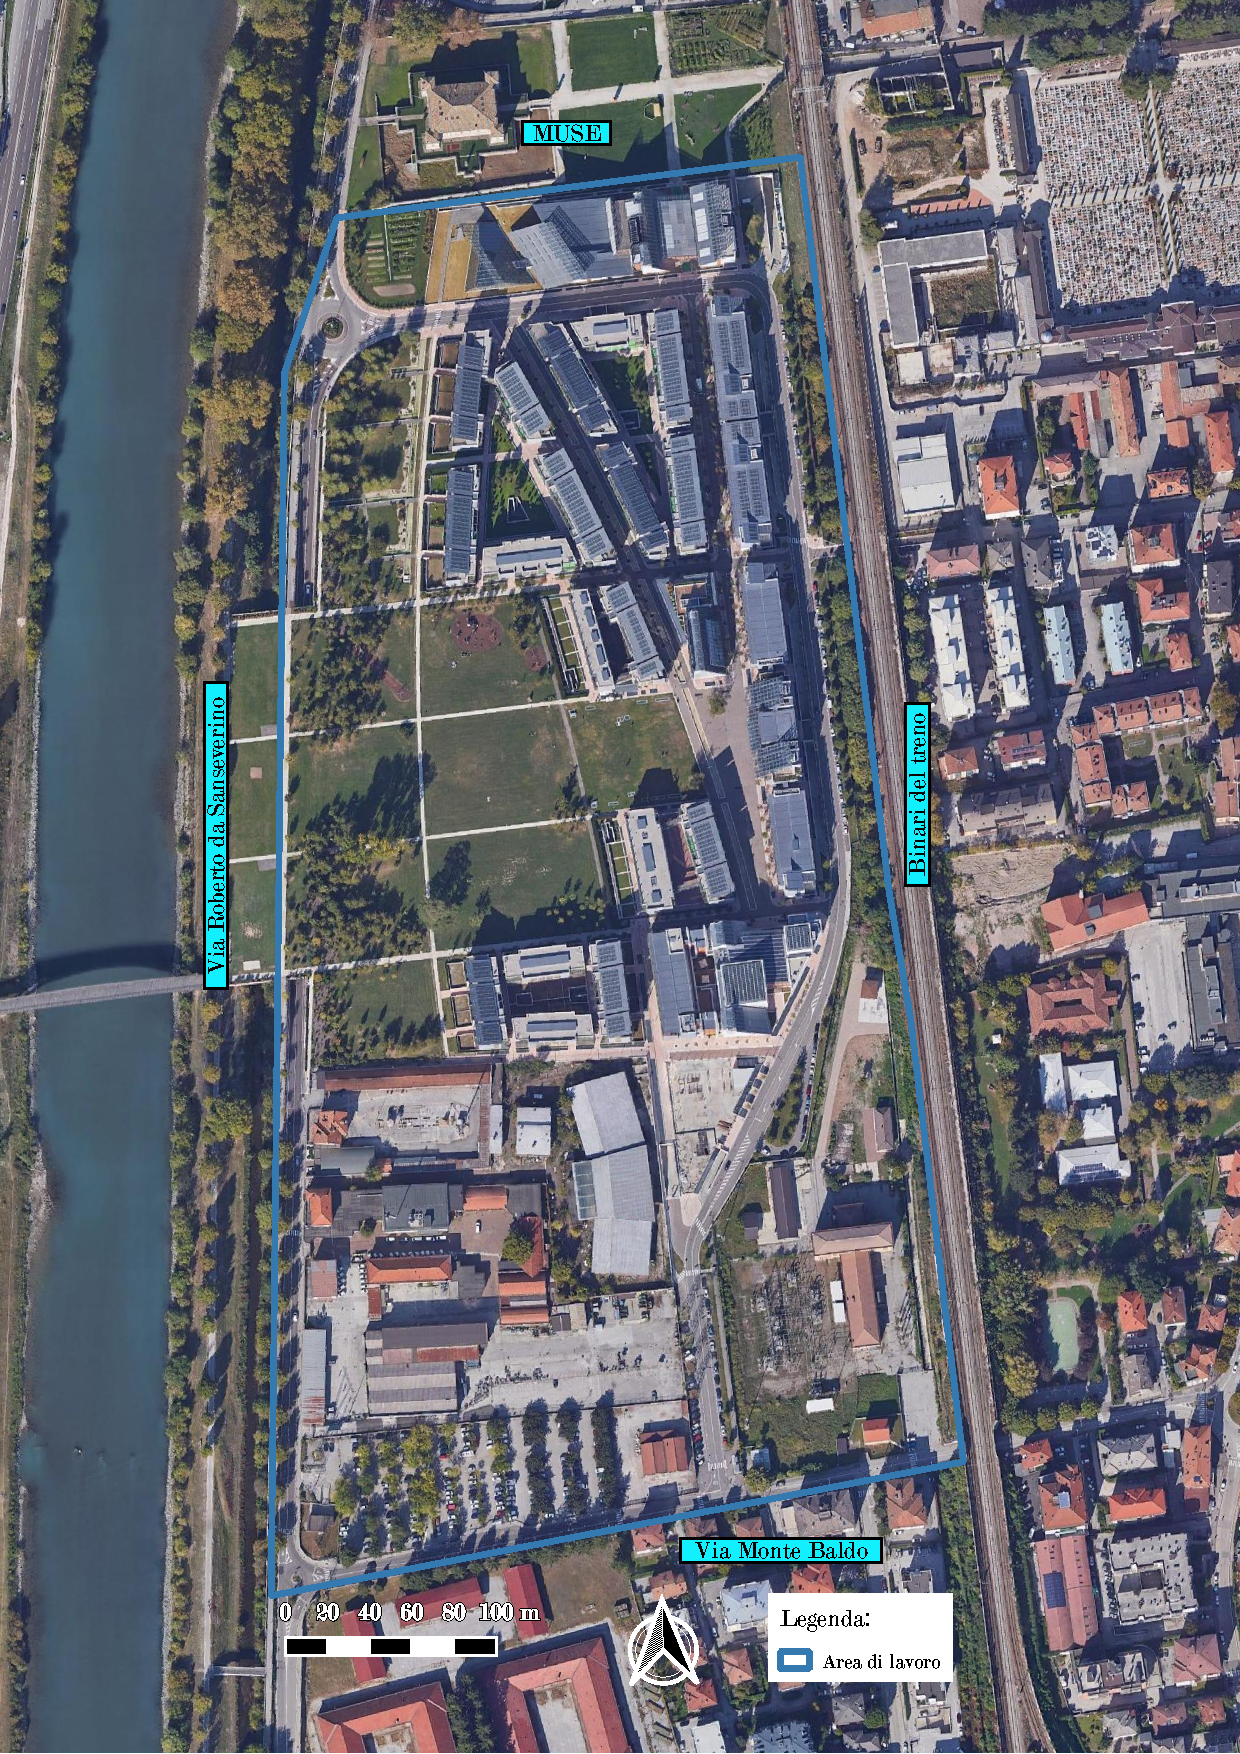
\includegraphics[trim=0cm 0cm 0cm 0cm,clip,frame,width=\textwidth]{IMG/inquadramento.pdf} 
    \caption{Inquadramento dell'area di lavoro}
    \label{fig:inquadramento}
    \end{figure}

\begin{equation}
    i = a \, t_p ^{n - 1}
\end{equation}
\begin{equation}
    CN = \frac{25400}{254 + S}
\end{equation}

\begin{equation}
    T_{\text{dry}} = \frac{3.125}{\sqrt{K_s}}
\end{equation}
Dove $T_{\text{dry}}$ sono i giorni che impiega il suolo completamente saturo a tornare secco e $K_s$ è la conduttività idraulica espressa in \si{inch\per\hour}.
\begin{equation}
    i_m = \frac{h(t_\text{fin}) - h(t_\text{in})}{\Delta t}
\end{equation}
\begin{equation}   
    h(t) = 
    \begin{cases}
        r \, a \left[ \left( \frac{t_p}{r}\right)^n - \left( \frac{t_p - t}{r}\right)^n  \right] & \text{se $t < t_p$}\\
        a \left[ r \left( \frac{t_p}{r}\right)^n + (1-r)\left( \frac{t_p - t}{1 - r}\right)^n  \right] & \text{se $t > t_p$}\\
    \end{cases}
\end{equation}
 


















\begin{landscape}
    \begin{figure}[htb]
        \centering
        \begin{tikzpicture}
            \begin{axis}[
                restrict x to domain=-0:1.5,
                height=15cm,
                width=21cm,
                grid=major,
                xlabel=Tempo trascorso dall'inizio della precipitazione \si{[\hour]},
                ylabel=Deflusso  \si{[\litre\per\second]},
                xtick = {0.5,1,1.5,2,2.5,3,3.5,4},
                %title= ,
                /pgf/number format/.cd,
                use comma,
                1000 sep={\,}
            ]
            \addplot +[mark=none,style=solid,color=red] table[x index=0,y index=1,header=false] {IMG/Total-Inflow/total_inflow_1min.txt};
            \addplot +[mark=none,style=solid,color=green!60!black] table[x index=0,y index=1,header=false] {IMG/Total-Inflow/total_inflow_2min.txt};
            \addplot +[mark=none,style=solid,color=magenta] table[x index=0,y index=1,header=false] {IMG/Total-Inflow/total_inflow_5min.txt};
            \addplot +[mark=none,style=solid,color=cyan] table[x index=0,y index=1,header=false] {IMG/Total-Inflow/total_inflow_10min.txt};
            \addplot +[mark=none,style=solid,color=orange] table[x index=0,y index=1,header=false] {IMG/Total-Inflow/total_inflow_15min.txt};
            \addplot +[mark=none,style=solid,color=teal] table[x index=0,y index=1,header=false] {IMG/Total-Inflow/total_inflow_30min.txt};
            \addplot +[mark=none,style=solid,color=violet] table[x index=0,y index=1,header=false] {IMG/Total-Inflow/total_inflow_45min.txt};
            \legend{1 min,2 min,5 min,10 min,15 min,30 min,45 min}    
            \end{axis}
        \end{tikzpicture}
        \caption{Deflusso del bacino}
        \label{fig:Ietogrammi}
    \end{figure}
\end{landscape}

\begin{landscape}
    \begin{figure}[htb]
        \centering
        \begin{tikzpicture}
            \begin{axis}[
                restrict x to domain=-0:4,
                height=15cm,
                width=21cm,
                grid=major,
                xlabel=Tempo trascorso dall'inizio della precipitazione \si{[\hour]},
                ylabel=Total Inflow  \si{[\litre\per\second]},
                xtick = {0.5,1,1.5,2,2.5,3,3.5,4},
                %title= ,
                /pgf/number format/.cd,
                use comma,
                1000 sep={\,}
            ]
            \addplot +[mark=none,style=solid,color=red] table[x index=0,y index=1,header=false] {IMG/Total-Inflow/total_inflow_5min_Chicago_25anni.txt};
            \end{axis}
        \end{tikzpicture}
        \caption{Andamento dello sforzo assiale agente sul pilastro P27 in funzione dell'altezza}
        \label{fig:IetogrammaFinale}
    \end{figure}   
\end{landscape}
\chapter{Rete di smaltimento delle acque meteoriche allo stato di progetto (con presenza
della rete di drenaggio)} \label{cap:ProgettoRete}
Analizzato quindi il deflusso dei sottobacini presenti nell'area di lavoro, si passa ora alla fase progettuale della rete di drenaggio. 
Tale progettazione sarà suddivisa in tre fasi principali in quanto si è voluto studiare tre casistiche di intervento: una rete di drenaggio composta da sole condotte e tombini, la precedente rete con l'aggiunta di sistemi di laminazione puntuale ed infine l'ulteriore aggiunta di sistemi di laminazione diffusi.

Dato il procedimento iterativo che compone ciascuna fase e il relativo aggiustamento dimensionale delle condotte (dovuto ad esempio  a sottobacini troppo piccoli e verifiche non soddisfatte, ecc) oppure della ri-progettazione della rete con solo i sistemi diffusi (per ottimizzare la dimensione delle condotte) e successiva aggiunta dei sistemi puntuali, si è voluto riportare in questo capitolo solo i risultati delle tre fasi principali sopra descritte e di  non riportare invece le fasi intermedie. %nell'appendice \ref{appendix:FasiIntermedie} a pagina \pageref{appendix:FasiIntermedie}. 

Di seguito verranno dapprima riportati i passaggi che contraddistinguono il dimensionamento e la verifica delle condotte in comune di ciascuna fase, per poi concentrarsi su ciascuna casistica riportando i risultati in forma per lo più tabellare o grafica.

\section{Procedimento per il progetto e verifica}
Data la necessità di conoscere il volume di riempimento delle condotte, la presenza di rigurgito o di moto in pressione è necessario cambiare le modalità di calcolo per la risoluzione della rete.
Nelle ipotesi di moto vario a superficie libera monodimensionale e con condotte di piccola pendenza, gradualmente variato e con fluido incomprimibile si utilizza ora il metodo dell'\emph{Onda Dinamica} che consiste nel considerare tutti i termini dell'equazione di De Saint Venant \ref{eq:saintvenant} relativa alla conservazione della quantità di moto, senza perciò trascurare quelli relativi al gradiente di pressione (come nel metodo dell'\emph{Onda Cinematica} visto prima in cui si era posto $S_0 = S_f$) e i termini inerziali. 
\begin{equation}
    \label{eq:saintvenant}
    \frac{\partial Q}{\partial t} + \frac{\partial}{\partial x} \left( \frac{Q^2}{A} \right) + g A \frac{\partial y}{\partial x} - g A (S_0 - S_f) = 0
 \end{equation}

\subsection{Profondità scavo}
Una volta scelto il percorso delle condotte e dei relativi tombini di collegamento, si deve fare in modo di allineare ciascuna di esse al cielo: 
questo per consuetudine italiana in cui si vuole avere più facilità di manutenzione e di posa degli strati in sommità delle condotte. 
Occorre quindi ipotizzare una pendenza delle condotte $i_g^{prog}$ di primo tentativo e successivamente calcolare la profondità di scavo (\emph{Max Depth}) data dalla differenza tra la quota del terreno e la quota di fondo.
La quota del terreno la si ottiene dai dati altimetrici dell'area (estratti usando QGIS), mentre la quota di fondo è data dalla somma, da valle a monte, dei dislivelli $\Delta h = i_g^{prog} \cdot L_{\text{condotta}}$ di ciascun tratto, partendo dalla quota nota dei recapiti finali (chiamati R1, R2, R3 nelle tabelle e nelle figure che seguiranno d'ora in poi).

Si ottiene così per ogni tratto una \emph{Max Depth} che deve essere
\begin{equation}
    \SI{1.5}{\metre} \lessapprox Max Depth \lessapprox\SI{6.5}{\metre}\quad ,
\end{equation} 
in modo di avere da un lato un ricoprimento minimo delle condotte tale che non si danneggino con il carico di veicoli, persone o intemperie;  dall'altro un ricoprimento contenuto da non avere costi di scavo troppo elevati. 
Per stare all'interno di tale intervallo si va ad agire sulla pendenza di progetto delle condotte o, eventualmente, su sistemi di rinforzo delle stesse.
\subsection{Diametro}
\begin{figure}[H]
    \centering
    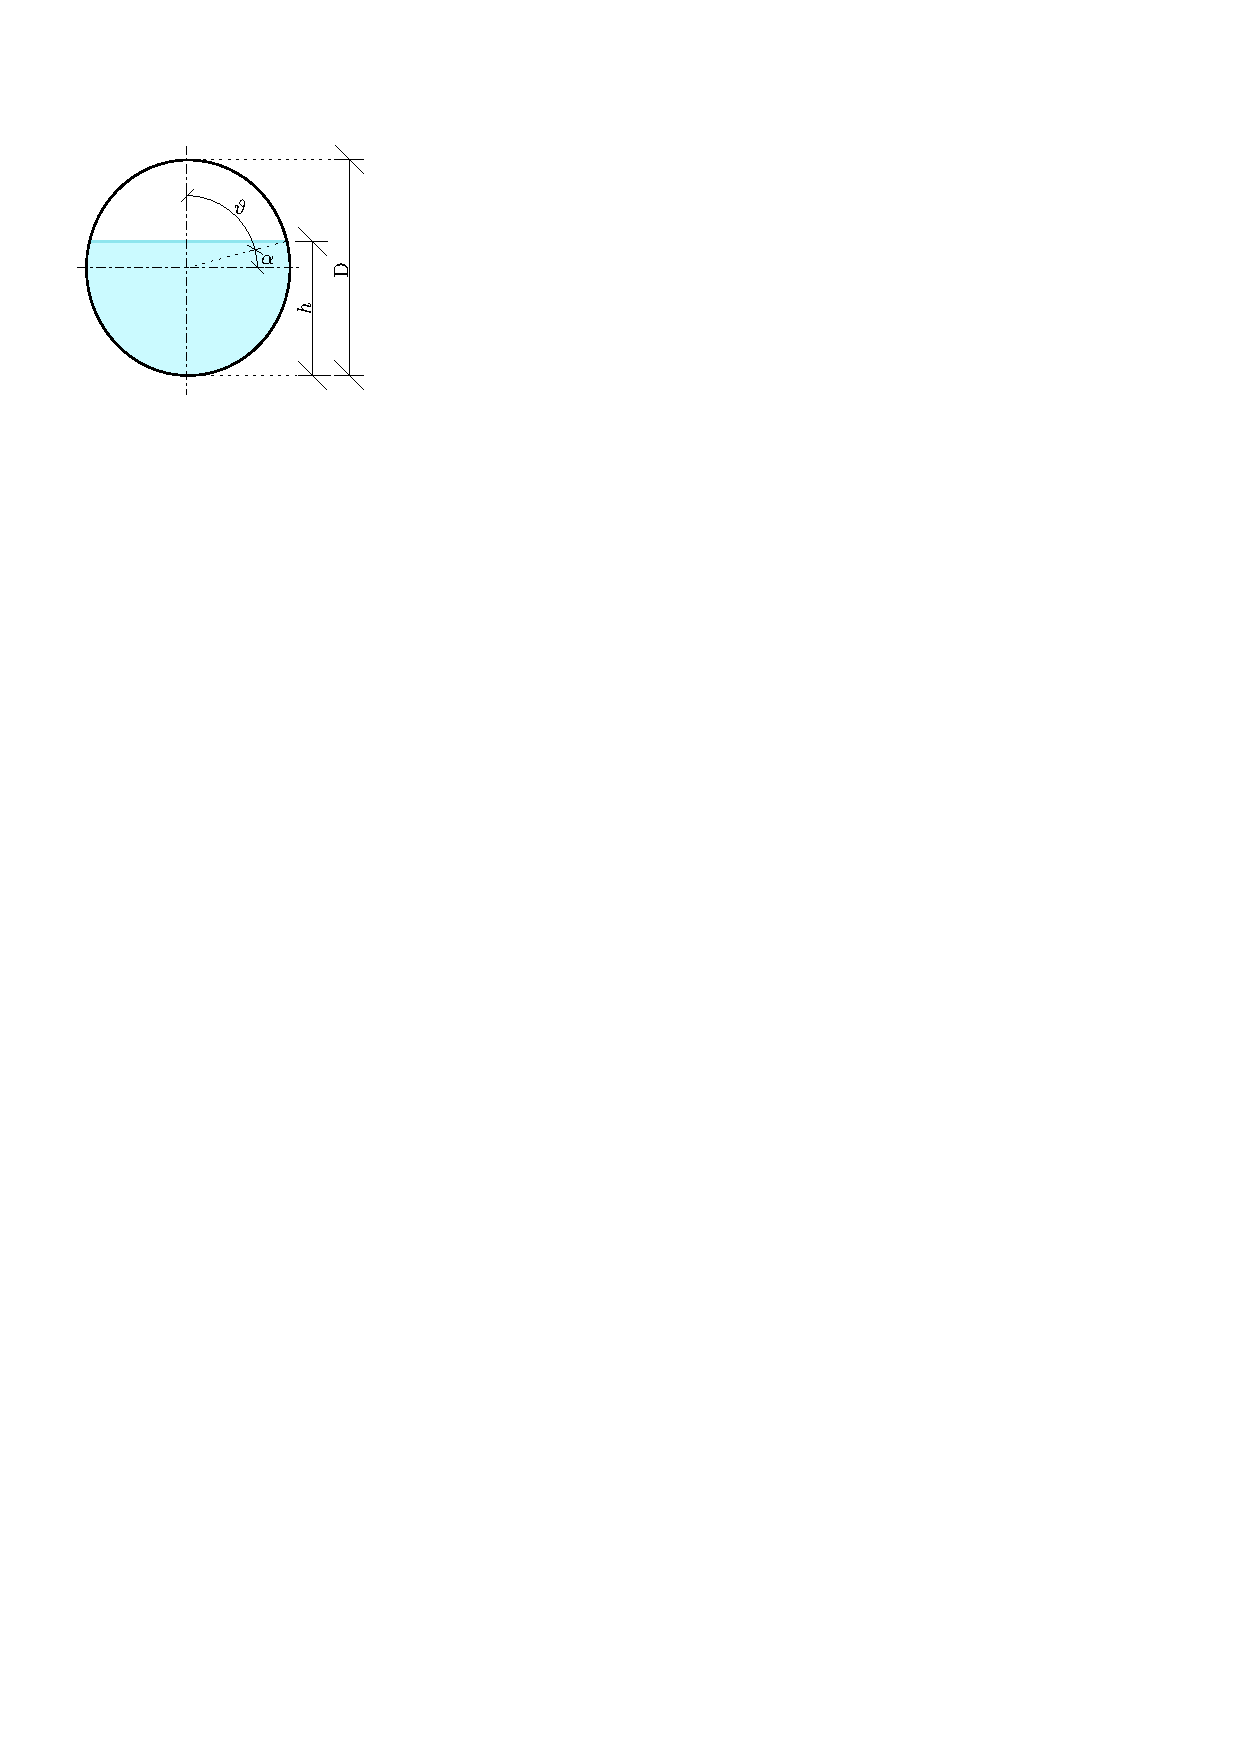
\includegraphics[]{IMG/RiempimentoCondotta.pdf}
\end{figure}
Con le ipotesi di moto sopra dette, si deve progettare la dimensione delle condotte facendo in modo di rispettare il loro riempimento così da rimanere all'interno delle ipotesi. 
Per questo si è imposto un riempimento ideale $\hat{\beta}$ del \SI{75}{\percent}
\begin{equation}
    \hat{\beta} = \frac{h}{D} = \SI{0.75}{} \quad .
\end{equation}

Dalla formula di Chézy, con la formulazione di Gauckler-Strickler, applicata al caso di condotte a sezione circolare e in riferimento alla nomenclatura di figura sopra, si ha tale legge che esprime la portata in funzione del riempimento:
\begin{equation}
    Q(\beta) 
    = A(\beta) \, k_s \, R^{\tfrac{2}{3}} \, i^{\tfrac{1}{2}} 
    = \frac{ D \, k_s \, f(\beta)^{\tfrac{5}{3}} \, i^{\tfrac{1}{2}} }{ 2^{\tfrac{13}{3}} \, g(\beta)^{\tfrac{2}{3}} }
\end{equation}
dove 
\begin{align}
    f(\beta) &= \pi - 2 \alpha - 2 (1 - 2 \beta) \cos(\alpha) \\
    g(\beta) &= \pi - 2 \alpha \\
    \alpha &= \arcsin(1 - 2 \beta)
\end{align}
e dalla quale si può ricavare il diametro minimo per il riempimento $\beta = \hat{\beta}$ fissato, avendo nota la portata $Q$ pari al deflusso a monte di tale condotta:
\begin{equation}
    D_{prog}(\hat{\beta}) = \frac{ 2^{\tfrac{13}{8}} \, g(\hat{\beta})^{\tfrac{1}{4}} }{     K_S^{\tfrac{3}{8}} \, f(\hat{\beta})^{\tfrac{5}{8}} } \frac{Q^{\tfrac{3}{8}}}{i^{\tfrac{3}{16}}} \quad .
\end{equation} 

Da tale diametro minimo se ne va a scegliere uno di sezione immediatamente superiore -- o al più di poco inferiore, a causa delle verifiche di riempimento nel capitolo successivo -- disponibile commercialmente.

Infine si calcola per ogni tratto la differenza di dimensione tra la condotta con diametro maggiore e tutte le altre, in modo da inserirle in SWMM e ottenere l'allineamento al cielo.

\subsection{Verifiche alle condotte}
Si deve ora verificare che le ipotesi fatte in fase progettuale siano state rispettate. 
Riguardo al riempimento ideale $\hat \beta$ imposto si deve controllare che il riempimento della condotta $\beta_\text{cond.}$ risulti 
\begin{equation}
    \SI{50}{\percent} \lessapprox \beta_\text{cond.} \lessapprox\SI{75}{\percent} \quad .
\end{equation}

Seguendo le indicazioni del Consiglio Superiore dei Lavori Pubblici la velocità dell'acqua all'interno delle condotte deve essere:
\begin{equation}
    \SI{0.5}{\metre\per\second} < V <  \SI{5}{\metre\per\second} \quad .
\end{equation}
Questo per non avere velocità troppo basse tali da formare dei sedimenti né velocità troppo elevate tali da danneggiare il materiale stesso delle condotte.
In realtà, per verificare che non si creino sedimenti nei periodi di non-precipitazione e rispettare il cosiddetto criterio di autopulizia, si è utilizzato anche un altro metodo che fa riferimento ad una tensione tangenziale al fondo $\tau$ minima oppure ad una pendenza del fondo (o idraulica) $i_f$ massima. 
Ovvero si deve avere:
\begin{equation}
    \label{eq:tau}
    \tau = \gamma \, R_H \, i_g > \SI{2}{\pascal}
\end{equation}
dove $\gamma$ è il peso specifico dell'acqua pari a \SI{1000}{\newton\per\metre\cubed}, $R_H$ è il raggio idraulico calcolato come rapporto tra area e perimetro bagnati, mentre $i_g$ è la pendenza geometrica delle condotte.  
\begin{align}
    R_H &= \frac{D}{4} \, \frac{1 - \sin(\vartheta)}{\vartheta} \\
    \vartheta &= 2 \, \arccos(1 - \beta_\text{cond.})
\end{align}
O analogamente
\begin{equation}
    i_g > i_f  
\end{equation}
in cui dalla \ref{eq:tau} si ha 
\begin{equation}
    i_f = \frac{\tau}{R_H \, \gamma} \biggr|_{\tau=\SI{2}{\pascal}}
\end{equation}    
mentre $i_g$ rimane la pendenza geometrica delle condotte, la quale deve essere comunque almeno del \SI{0.5}{\percent}.






\section{Progetto}
\label{cap:ProgettoCondotte}
Il progetto della rete di drenaggio prevede tre rami principali ciascuno composto da altrettanti recapiti finali affluenti al canale Adigetto. 
I rami principali delle condotte, visibili nel dettaglio in figura \ref{fig:Condotte} nella fase progettuale finale, sono posti a nord, centro e sud dell'area di studio in concomitanza dei tre recapiti $R1$, $R2$, $R3$ posti a quota prefissata di \SI{184.00}{}, \SI{183.70}{} e \SI{183.50}{\metre}.
\begin{figure}[p]
    \centering
    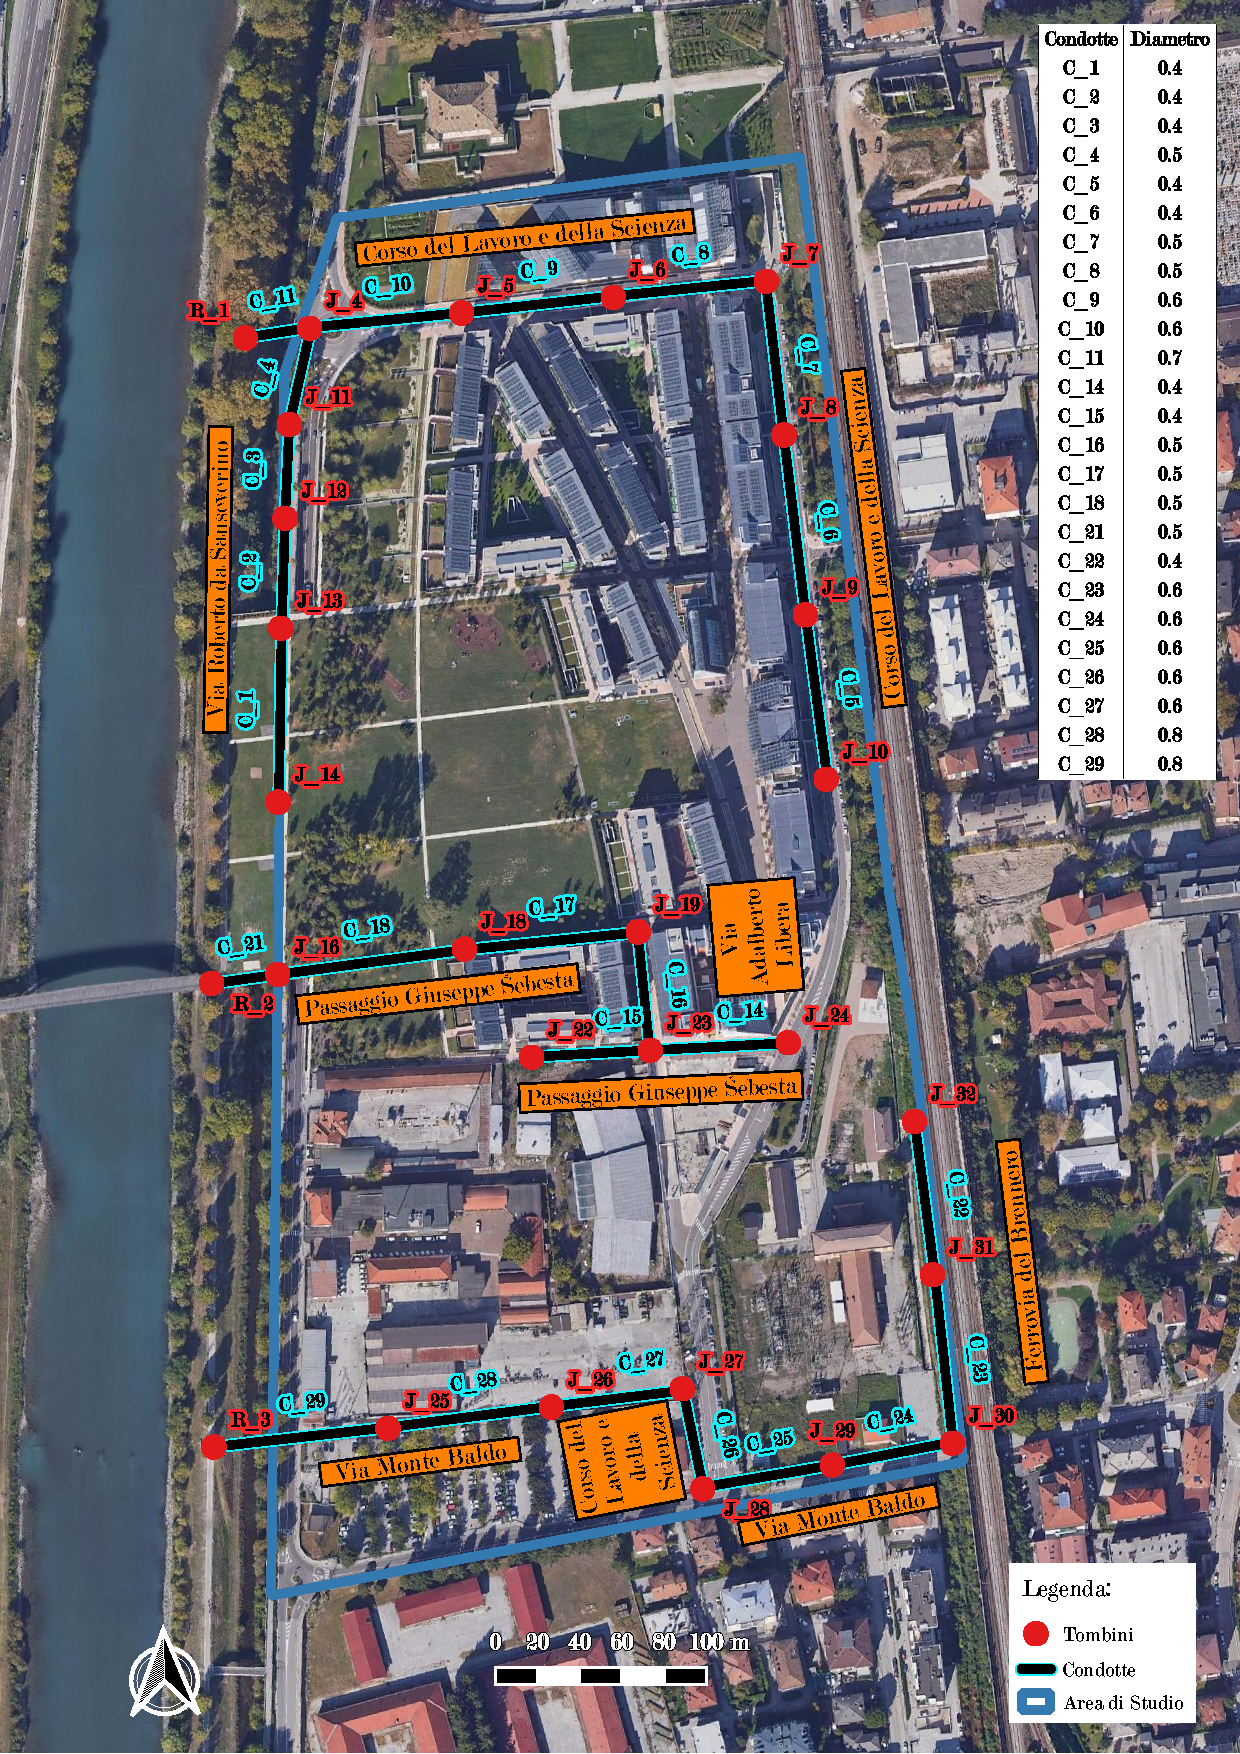
\includegraphics[trim=0cm 0cm 0cm 0cm,clip,frame,width=0.9\textwidth]{IMG/Nomenclatura_condotte.pdf} 
    \caption{Posizionamento e nomenclatura della rete di drenaggio con indicazione del deflusso dei sottobacini}
    \label{fig:Condotte}
\end{figure}

Il percorso delle reti cerca di sovrapporsi a strade o vicoli pre-esistenti in modo da non aumentare l'impatto ambientale e visivo. 
Cerca inoltre di attraversare ogni sottobacino per confluire ad ognuno il deflusso in un rispettivo tombino, idealmente a monte della condotta. 
In questo modo si riesce a dimensionare con maggiore efficacia le tubazioni. 
In aggiunta le condotte devono essere interrotte da un tombino d'ispezione e non divenire più lunghe di \SI{100}{\metre}.

Per tutte le componenti della rete è stato usato calcestruzzo armato senza nessun particolare rivestimento per cui, avendo condotte circolari con pareti non perfettamente lisce, si è scelto un coefficiente di Gauckler-Strickler $k_s$ pari a \SI{80}{\metre\tothe{1/3}\per\second} -- equivalente ad un numero di Manning $n$ di \SI{0.0125}{\metre\tothe{1/3}\second}, avendo usato il software SWMM di concezione anglosassone.

Il procedimento descritto nel paragrafo precedente è alla base dei dati tabulari di seguito esposti.  
Nella tabella \ref{tab:Nodi_nodes-mod} è riportata la profondità di scavo in base alla pendenza scelta delle condotte. 
Nella tabella successiva si ha il calcolo del diametro di progetto e la relativa scelta del diametro commerciale, facendo attenzione alle verifiche di riempimento e di velocità visibili invece nell'ultima tabella a seguire.

Nel tombino $J13$ non riuscendo a rispettare la profondità di scavo minima di \SI{1.5}{\metre}, ma essendo invece di \SI{0.85}{\metre}, si prevede una soletta armata sopra il tombino e lungo parte delle due condotte ad esso collegate per evitare la rottura a taglio del calcestruzzo dovuto a carichi sovrastanti. 

Nel caso delle condotte 18 e 21 si è scelto un diametro commerciale maggiore del dovuto per non avere scalini con le condotte a monte nei quali si accumulerebbero detriti. 

In figura \ref{fig:ProfiliProgettoCondotte} a pagina \pageref{fig:ProfiliProgettoCondotte} è mostrato l'andamento del pelo libero dell'acqua all'interno delle condotte nel momento di massimo picco.

Come si nota dalla figura \ref{fig:Condotte} alcuni sottobacini sono stati in realtà considerati uniti, facendo convogliare il deflusso nello stesso tombino.
Questo perché con la disposizione iniziale non si soddisfava la verifica del riempimento minimo.
%La disposizione iniziale si può vedere in appendice \ref{appendix:FasiIntermedie} nella fi e LE TABELLE SBAGLIATE a pagina TOT.

\TabellaNodi{Profondità di scavo dei tombini e pendenza progettuale delle condotte -- Progetto base con solo condotte}{tab:Nodi_nodes-mod}{IMG/Nodi-nodes-mod.tex}
\TabellaDiametriCondotte{Diametro commerciale e offset per l'allineamento al cielo -- Progetto base con solo condotte}{tab:Diametri_conduct-mod}{IMG/Diametri-conduct-mod.tex}
\TabellaVerificheLinkFLow{Verifiche massima velocità, riempimento e criterio di autopulizia -- Progetto base con solo condotte}{tab:LinkFlow_Verifiche-MOD}{IMG/LinkFlow-Verifiche-MOD.tex}
\begin{figure}[p]
    \centering
    % \subfloat[][\emph{Campata 1\label{fig:MomentiUnitariA}}]
    \subfloat[][\emph{Ramo di condotte tra il recapito finale 1 ed il tombino $J10$}]{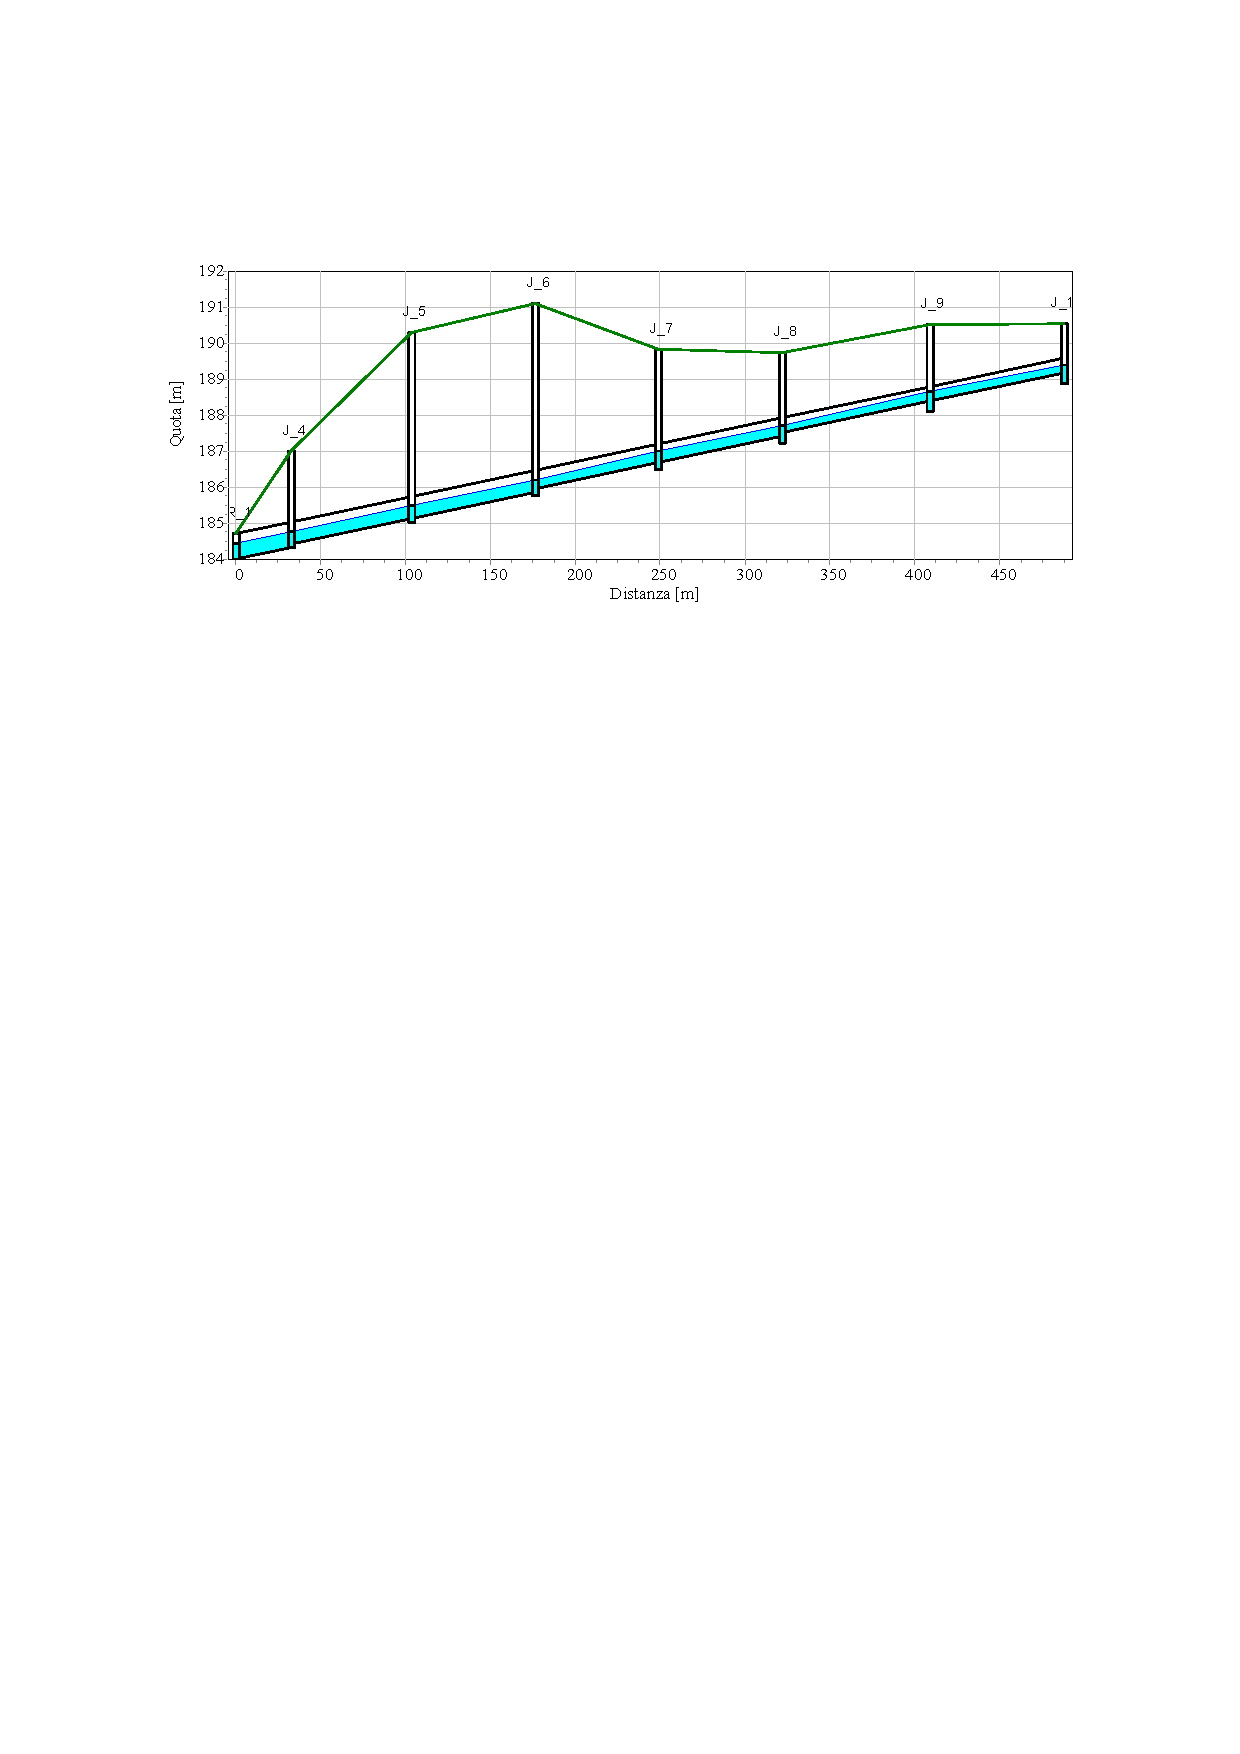
\includegraphics[width=\textwidth]{IMG/ProgettoCondotte_profiloA.pdf}} \\
    \subfloat[][\emph{Ramo di condotte tra il recapito finale 2 ed il tombino $J24$}]{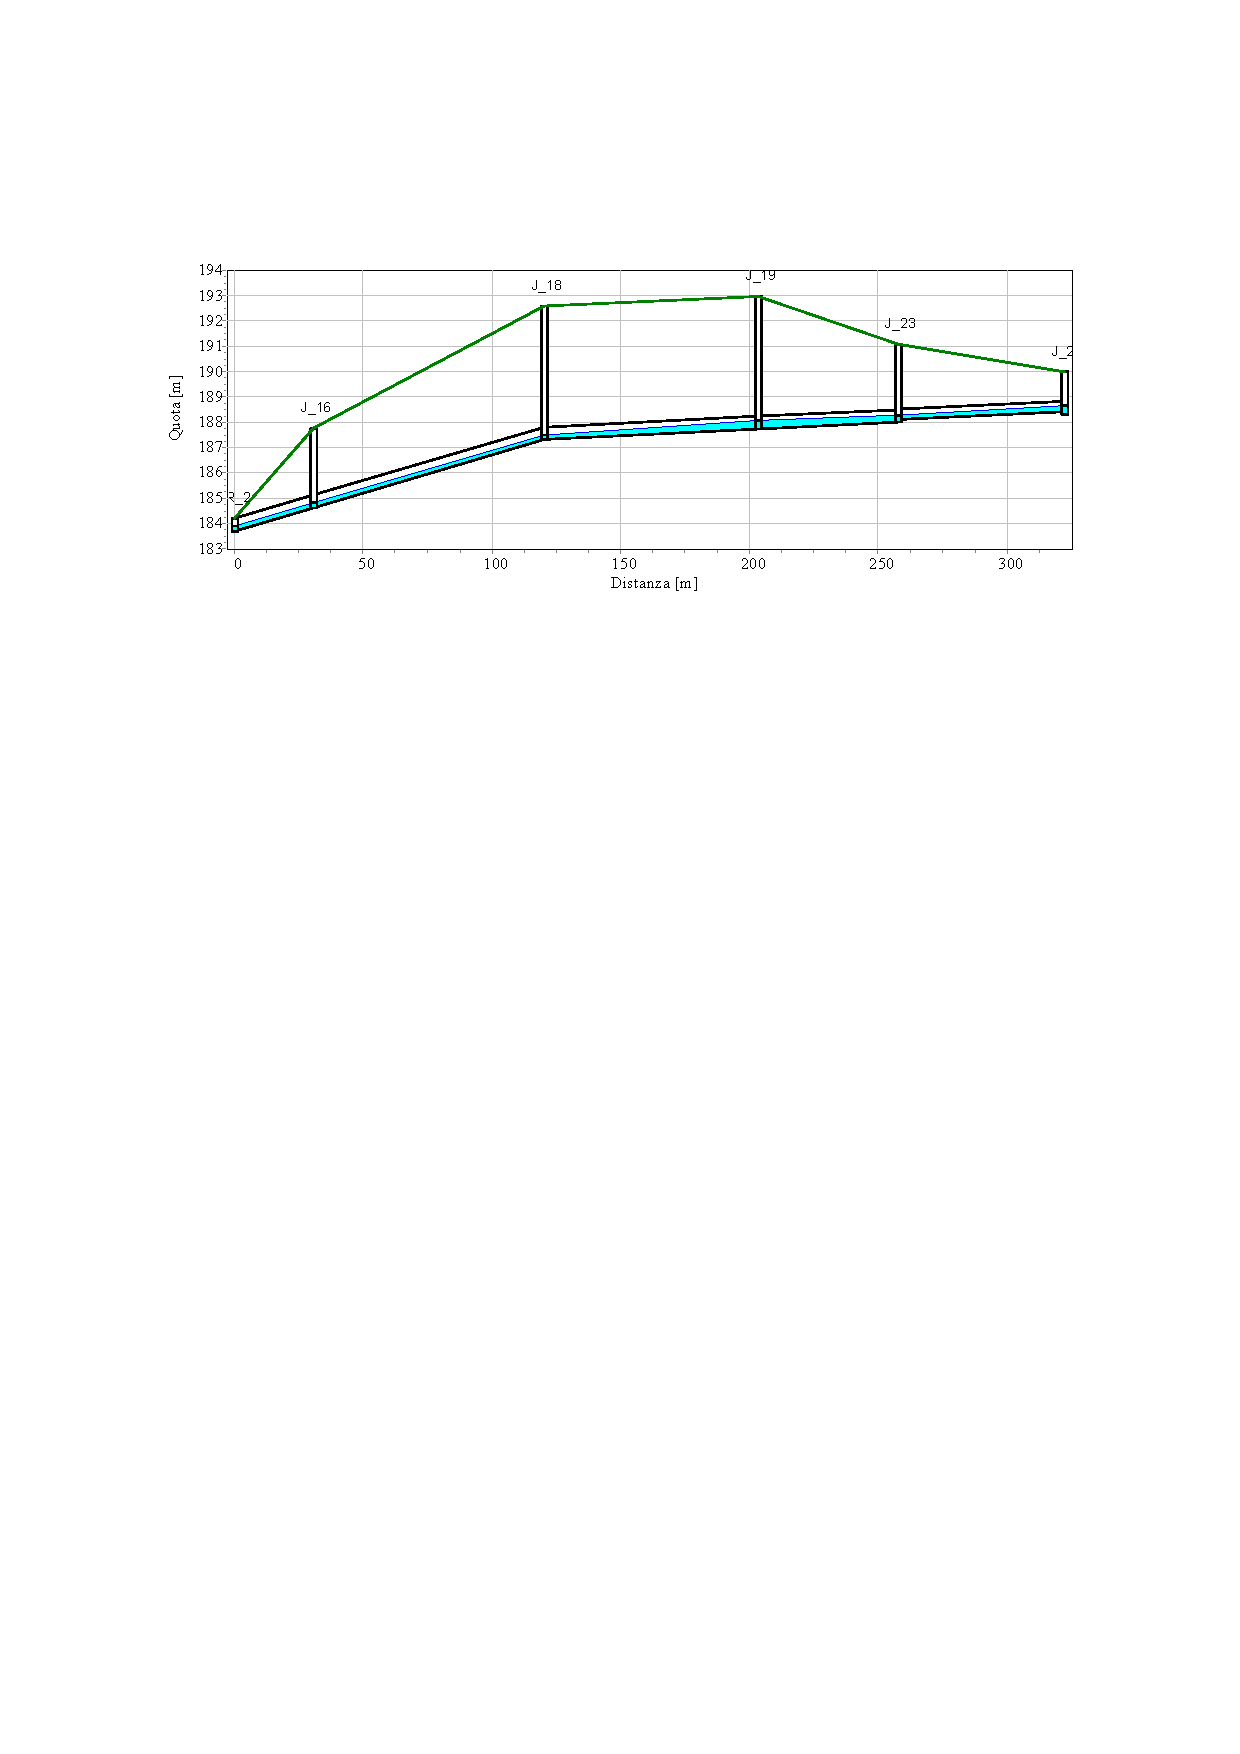
\includegraphics[width=\textwidth]{IMG/ProgettoCondotte_profiloB.pdf}} \\
    \subfloat[][\emph{Ramo di condotte tra il recapito finale 3 ed il tombino $J32$}]{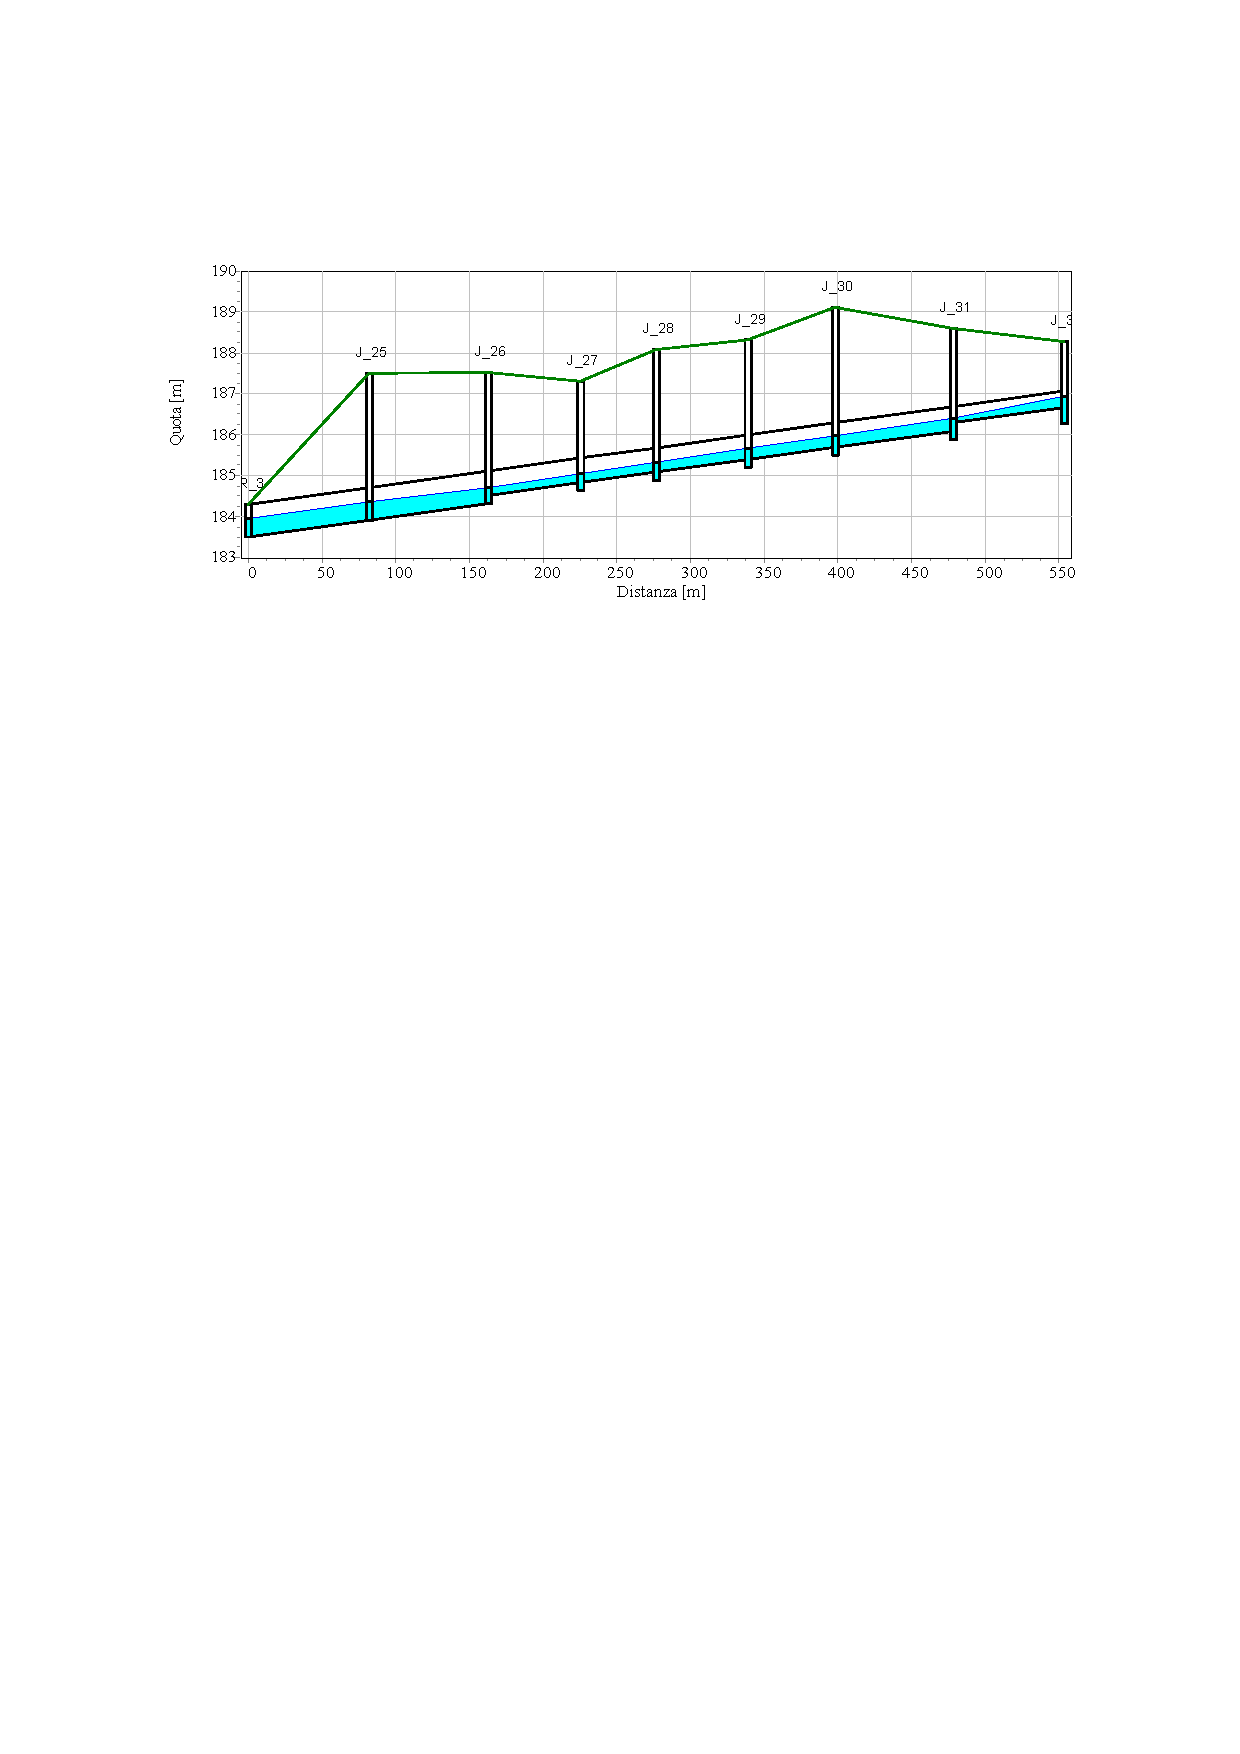
\includegraphics[width=\textwidth]{IMG/ProgettoCondotte_profiloC.pdf}}
\caption{Andamento del pelo libero dell'acqua all'interno delle condotte nell'instante di massimo picco -- Progetto base con solo condotte}
\label{fig:ProfiliProgettoCondotte}
\end{figure}




\end{document}